\documentclass{article}

\usepackage{minitoc}
\usepackage{tabularx}
\usepackage{booktabs}
\usepackage{graphicx}
\usepackage{hyperref}
\usepackage{xcolor}
\usepackage{blkarray}
\usepackage{amsthm, amssymb, amsmath}
\usepackage{caption}
\usepackage{subcaption}
\usepackage{multirow}
\usepackage[ruled,vlined]{algorithm2e}

% \usepackage{natbib}
% \bibliographystyle{abbrvnat}
\bibliographystyle{abbrv}

\theoremstyle{definition}
\newtheorem{definition}{Definition}[section]
\newtheorem{theorem}{Theorem}[section]
\newtheorem{lemma}[theorem]{Lemma}
\newtheorem{conjecture}[theorem]{Conjecture}
\newtheorem{corollary}{Corollary}[theorem]

\usepackage[margin=2.5cm, includefoot, footskip=30pt]{geometry}
\pagestyle{plain}
\setlength{\parindent}{0em}
\setlength{\parskip}{1em}

\renewcommand{\baselinestretch}{1}

\usepackage{standalone}

\newtheorem{proposition}{Proposition}

\title{Reactive strategies with longer memory}

\author{Nikoleta E. Glynatsi, Ethan Akin, Martin Nowak, Christian Hilbe}
\date{}

\begin{document}

\maketitle

\begin{abstract}

In the following, we study repeated games and the strategies players can
employ in these games. Famously, in repeated games it is assumed that
strategies that use the past history can be adopted. Here we focus on such a
set, called reactive strategies. In comparison to previous studies this work
explores higher memory strategies, greater than one compared to the majority
of the works in the literature.

We demonstrate how this set of strategies have an immediate effect on the
co-player and show that a history that is not shared does not benefit the
longer strategy.

We then characterise partner strategies, which are strategies ensuring mutual
cooperation without being exploited. A recipe for evolutionary stability. We
show that the class of Tit For Tat and Generous Tit For strategies even the
delayed versions of these strategies are partner strategies.

For memory lengths of two and three we characterize all partner strategies
amongst the reactive set. The conditions are simple and yet newly found. For a
specific class of reactive counting strategies, counting of
defections/defections instead of remembering the actual occurrence of the
action, we can characterize partner strategies in all memory lengths.

We further test the evolutionary properties of partner strategies in higher
memory. The results show that.


\end{abstract}

\section{Introduction}

The emergence of cooperation can be explained by direct reciprocity, where
individuals provide assistance to each other through repeated interactions~\cite{axelrod:AAAS:1981,
nowak:Science:2006, sigmund2010}. Traditionally, researchers have adopted the repeated prisoner's dilemma
as a conceptual framework for capturing the dynamics of direct reciprocity. In
this model, two individuals, often referred to as players, engage in multiple
rounds of interaction. During each round, both players face the decision of
whether to cooperate or defect. Mutual cooperation results in more favorable
outcomes compared to mutual defection, but the self-interest of each individual
frequently leads to the temptation to defect.

Strategies employed in the repeated prisoner's dilemma can become notably
complex. Examples of sophisticated strategies include those that consider the
entire past history of interactions when deciding whether to cooperate in the
next round, or those that take into account additional information derived from
the history, such as the number of defections that occurred by both players~\cite{harper:PLOSONE:2017,
knight:PLOSONE:2018, li:NatureCompSci:2022}.
Empirical studies have shown that human behavior often demonstrates conditional
cooperation in repeated games~\cite{fischbacher:AER:2010, rand:Elsevier:2013,
grujic:ScientificReports:2014}. Moreover, several experiments suggest
that the complexity of human strategies is limited. However, it is important to
note that some of these assumptions have also been challenged and debunked.

Theoretical models have primarily focused on one side, namely, they have
extensively concentrated on naive subjects who do not remember anything beyond
the outcome of the very last round~\cite{nowak:Nature:1992,
glynatsi:scientific:2020, press:PNAS:2012, stewart:scientific:2016,
nowak:Nature:1993, kraines:elsevier:2000, imhof:ProceedingsB:2010,
baek:scientific:2016, hilbe:PNAS:2013, chen:PNASnexus:2023, hilbe:Nature:2018,
akin:EGADS:2016}.
These strategies are known as memory-1 strategies and can be described by four
parameters, specifically, the probabilities of cooperating after each possible
outcome of the last round. Extensive research has centered on these strategies,
allowing us to explore the entire space and characterize when strategies are
Nash equilibria. Furthermore, we have uncovered other interesting properties of
these strategies. Examples include zero-determinant strategies, which constitute
a set of strategies capable of enforcing a linear relationship between the
payoffs of the two players~\cite{press:PNAS:2012}, equalizers, a set of
strategies that equalize the co-player's score, assigning it a predetermined
value independent of the co-player's strategy~\cite{hilbe:PNAS:2013}, and
partner strategies, which ensure mutual cooperation without
exploitation~\cite{hilbe:Nature:2018}.

Attempts have been made to extend these results to strategy sets that consider
more turns, and equivalently more memory. Notable works include those
of~\cite{hilbe:PNAS:2017, ueda:RSOP:2021}. Specifically, the
work~\cite{ueda:RSOP:2021} characterized zero-determinant strategies for
memory-two strategies, and~\cite{hilbe:PNAS:2017} managed to characterize
subsets of memory-$n$ partner strategies. Exploring higher memory spaces is not
a trivial issue. While a memory-1 strategy can be defined by four parameters, a
memory-2 strategy is defined by 16, and a memory-3 strategy is defined by 256
parameters. This makes the space of strategies in higher memory spaces
intractable.

Herein, we approach higher memory strategies by focusing on a specific set of
memory$-n$ strategies that react only to one player's actions. There can be two
such sets. One is reactive strategies, which only consider the co-player's
actions in the previous turns. Another reactive class is that of self-reactive
strategies, which consider the focal player's actions. However, it can easily be
shown that in the case of self-reactive strategies, the Nash equilibrium is that
of always defect. As such, we focus on reactive strategies.

We manage to characterize all partner strategies amongst the reactive-2 and
reactive-3 sets.

To assess whether a given strategy class is favourable to the evolution of
cooperation, we consider the Moran process in a finite population of players.

\section{Model}

\textbf{Repeated Game.}
We consider an infinitely repeated game with two players. In each round, player 1
and player 2, can choose to cooperate ($C$) or to defect ($D$). If both players
cooperate, they receive a payoff $R$ (the reward for mutual cooperation), and if
both players defect, they receive a payoff $P$ (the punishment for mutual
defection). If one player cooperates, the cooperative player receives the
sucker's payoff $S$, and the defecting player receives the temptation payoff
$T$. We assume that the payoff are such that $T > R > P > S$ and $2 R > T + S$.
This game is known as the Prisoner's Dilemma. Here, we
employ a specific parametrization of the Prisoner's Dilemma, where cooperation
implies incurring a cost $c$ for the co-player to derive a benefit $b > c$.
Consequently, the payoffs are defined as follows: \(R = b - c, S = -c, T = b, P =
0\). In the Appendix, we present results applicable to the general Prisoner's
Dilemma.

We assume in the following, that the players' decisions only depend on the
outcome of the previous $n$ rounds. To this end, an {\it $n$-history for player
$i \in \{1, 2\}$} is a string $h^i=(a^i_{-n},\ldots,a^i_{-1})\!\in\!\{C,D\}^n$
where an entry $a^i_{-k}$ corresponds to player $i$'s action $k$ rounds ago. Let
$H^i$ denote the space of all $n$-histories for player $i$ where set $H^i$ contains
$|H^i|=2^{n}$ elements. A {\it reactive$-n$ strategy} for player 1 is a vector
$\mathbf{p}=(p_h)_{h\in H^2} \in [0, 1]^{n}$. Each entry $p_h$ corresponds to
the player's cooperation probability in the next round, based on the co-player's
actions in the previous $n$ rounds. Therefore, reactive-$n$ strategies
exclusively rely on the co-player's $n$-history, independent of the focal
player's own actions. For \(n=1\), this definition of reactive-\(n\) strategies
recovers the typical format of reactive-1 strategies~\cite{baek:scientific:2016, wahl:JTB:1999, mcavoy:PRSA:2019},
\(\mathbf{p}=(p_C, p_D,)\).

Another class of strategies we will be discussing in this work are, {\it
self-reactive-$n$} strategies which only consider the focal player's own
$n$-history, and ignore the co-player's. Formally, a self-reactive-$n$ strategy
for player 1 is a vector $\mathbf{\tilde{p}} = (\tilde{p}_h)_{h \in H^1} \in [0,
1] ^ {n}$. Each entry $\tilde{p}_h$ corresponds to the player's cooperation
probability in the next, depending on the player's own actions in the previous
$n$ rounds. We say that a reactive or self-reactive strategy is pure if all the
entries of the strategy are either 0 or 1. We refer to the set of all pure
self-reactive strategies as $\tilde{P}_n$.

\begin{figure}[h!]
  \centering
  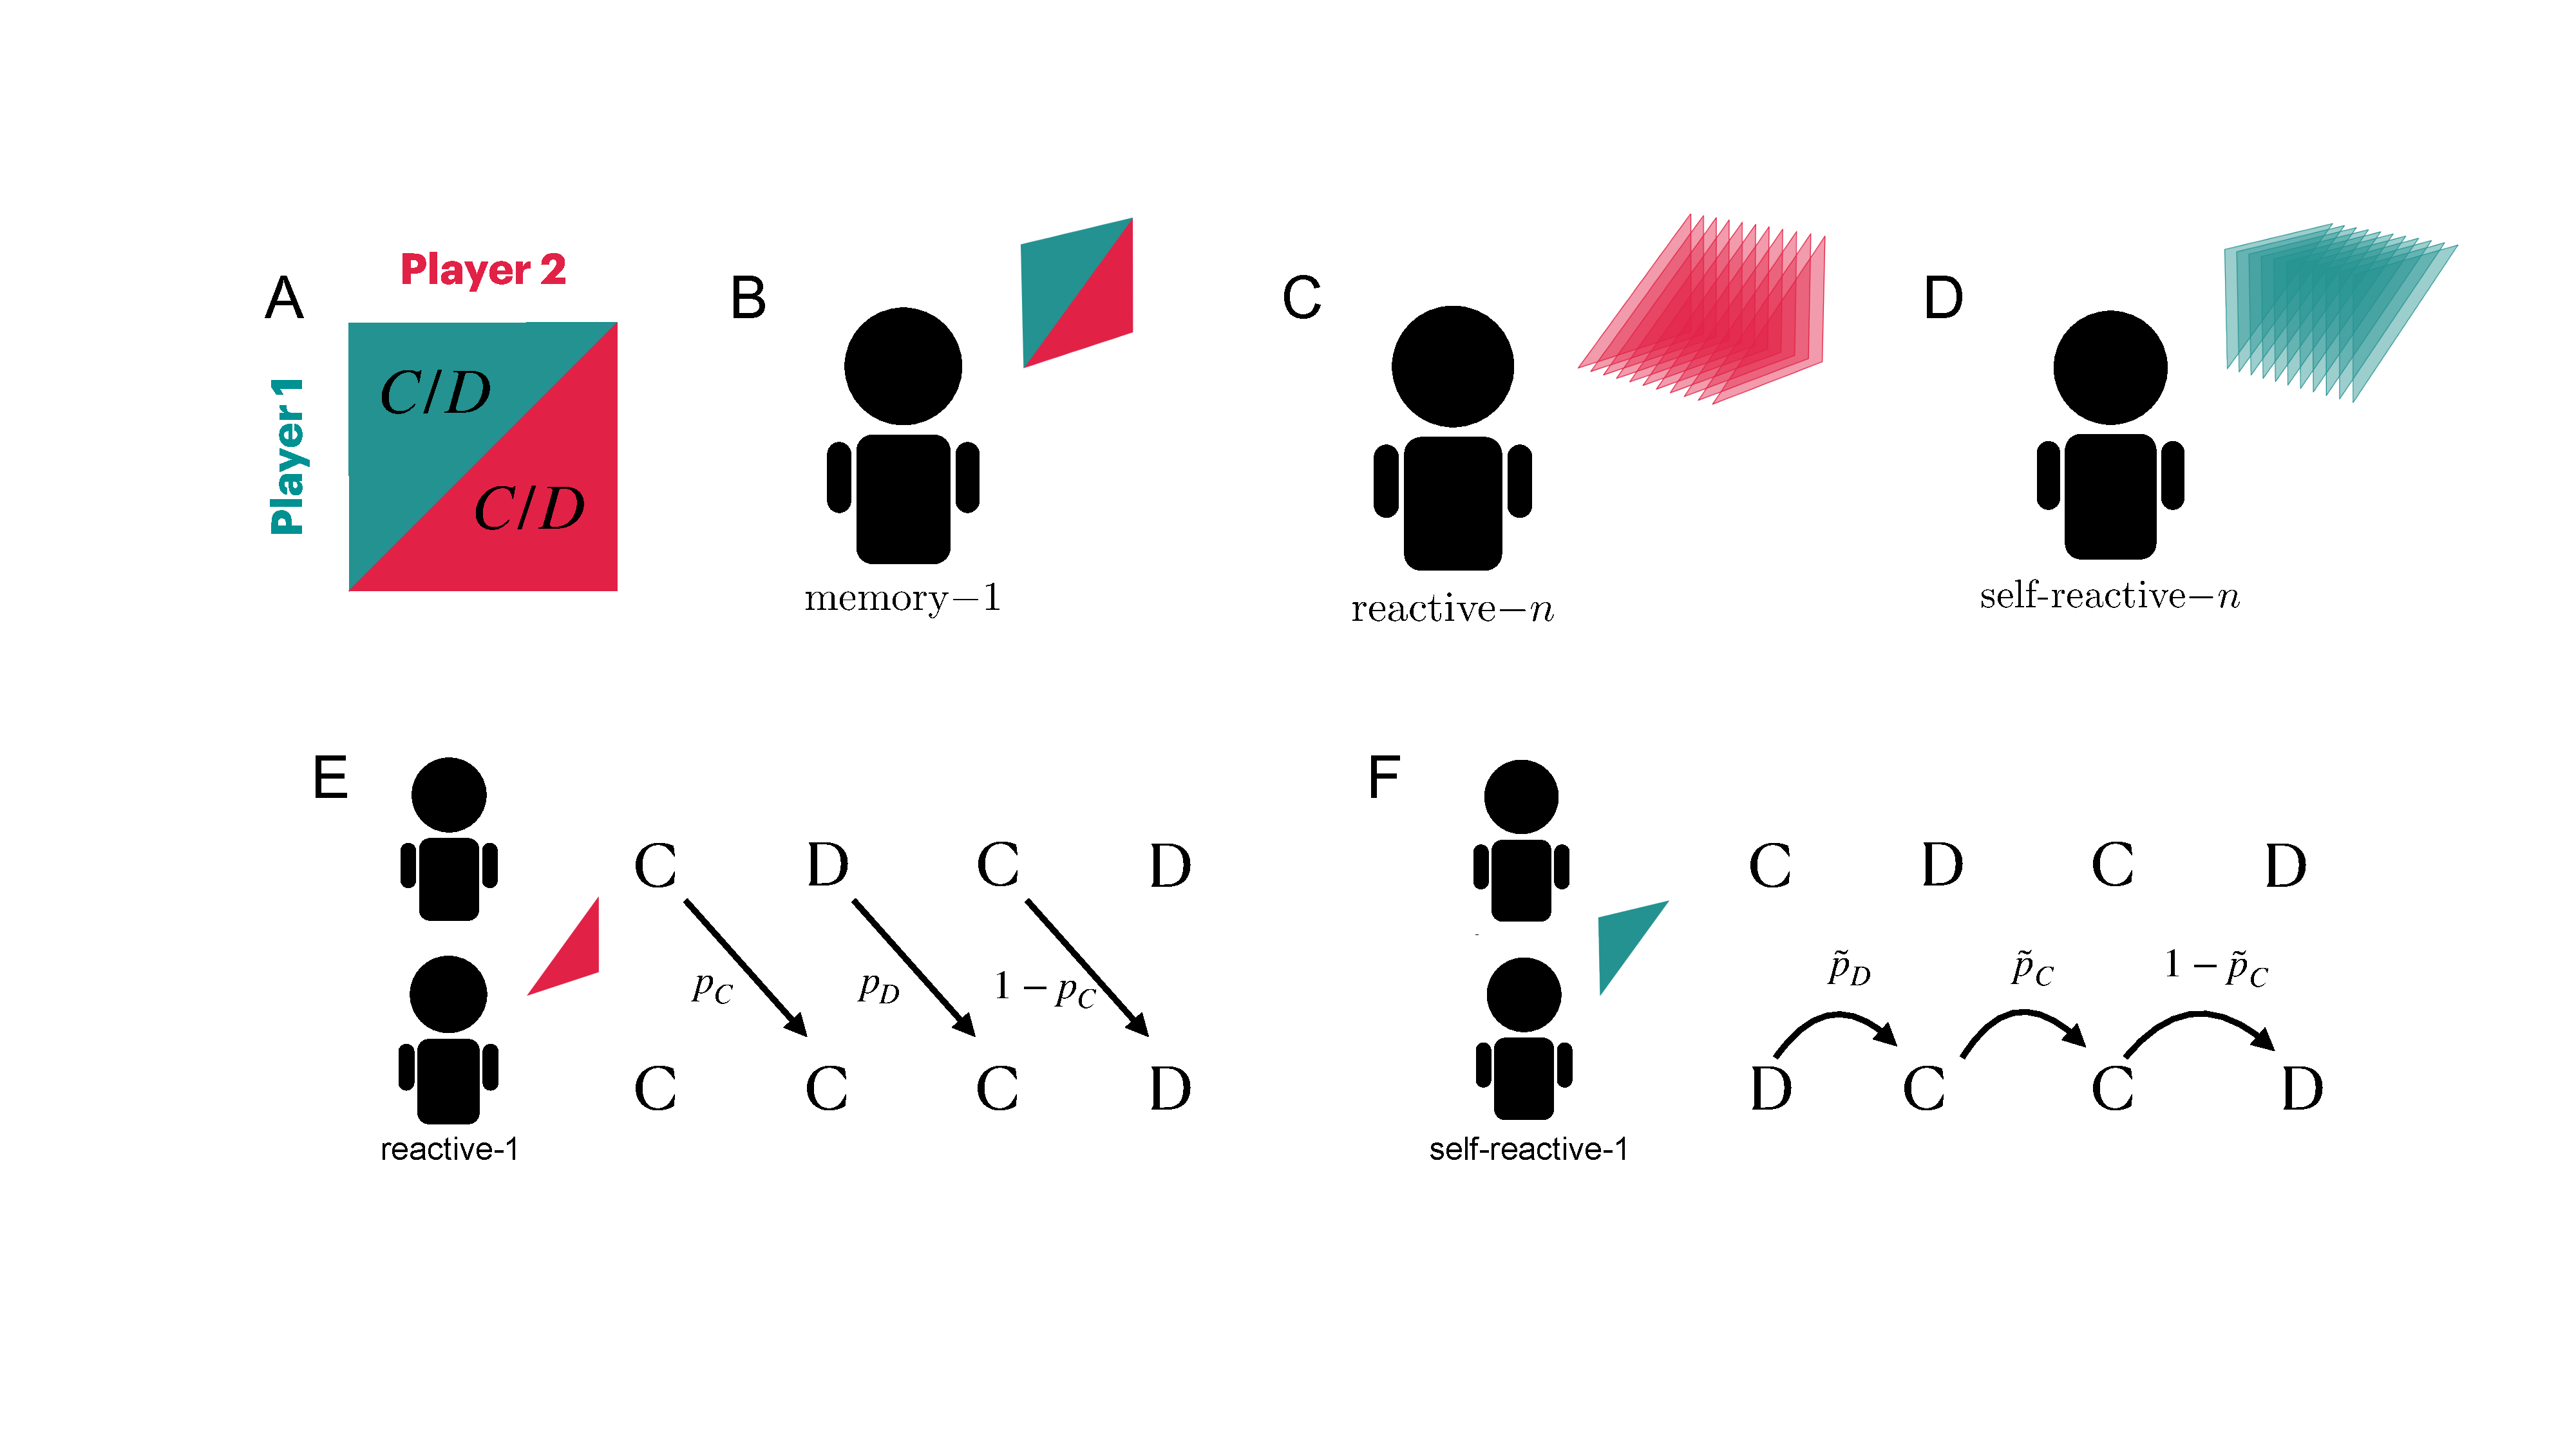
\includegraphics[width=\textwidth]{figures/conceptual_figure_model.pdf}
  \caption{\textbf{Model.}
  \textbf{a.} In each turn of the repeated game, players 1 and 2 decide on an action,
  denoted as $C$ (cooperate) or $D$ (defect), respectively. We assume, that the information that a
  player can use in subsequent turns is limited to the actions taken by both
  players in the current turn.
  \textbf{b.} Memory-$1$ strategies, a well-studied set of strategies, utilize the
  actions of both players in the previous turn to make decisions. In the graphical
  representation of memory-$1$ strategies, we use a single square to illustrate this
  concept.
  \textbf{c.} This work primarily focuses on reactive-$n$ strategies, which take
  into account only the actions of the co-players.
  \textbf{e.} For the case of $n = 1$, a reactive-$1$ strategy is represented as a vector $\mathbf{p} =
  (p_C, p_D)$, where $p_C$ is the probability of cooperating given that the co-player
  cooperated, and $p_D$ is the probability of cooperating given that the co-player
  defected. In the example shown, the bottom player employs a reactive-$1$ strategy.
  They cooperate with a probability $p_C$ in the second round because the co-player
  cooperated in the first round. In the second round, the player cooperates with a
  probability $p_D$ since the co-player previously defected. Finally, the player
  defects in the third round with a probability of $1 - p_C$, considering that the
  co-player cooperated.
  \textbf{d.} Another set of strategies we consider is that of self-reactive-$n$
  strategies, which rely solely on a player's own previous $n$ actions.
  \textbf{f.} For the case of $n = 1$, a self-reactive-$1$ strategy is represented
  as a vector $\mathbf{\tilde{p}} = (\tilde{p}_C, \tilde{p}_D)$, where
  $\tilde{p}_C$ is the probability of cooperating given that the player's last
  action was cooperation, and $\tilde{p}_D$ is the probability of cooperating
  given that the player's last action was defection. In the example shown, the
  bottom player employs a self-reactive-$1$ strategy. They cooperate with a
  probability $\tilde{p}_D$ in the second round given that they defected in the
  first. In the second round, the player cooperates with a probability
  $\tilde{p}_C$ since they cooperated in the previous round. Finally, the player
  defects in the third round with a probability of $1 - \tilde{p}_C$, considering
  that they cooperated in the previous round.}
\end{figure}

\textbf{Evolutionary process.} To examine the evolutionary properties of
reactive strategies, we perform an evolutionary study based on the framework of
Imhof and Nowak~\cite{imhof:royal:2010}. The framework considers a population
of size \(N\) where initially all members are of the same strategy. In our case
the initial population consists of unconditional defectors. In each elementary
time step, one individual switches to a new mutant strategy. The mutant strategy
is generated by randomly drawing cooperation probabilities from the unit
interval \([0,1]\). If the mutant strategy yields a payoff of \(\mathbf{s}_{M, k}\),
where \(k\) is the number of mutants in the population, and if residents get a
payoff of \(\mathbf{s}_{R, k}\), then the fixation probability \(\phi_{M}\) of the
mutant strategy can be calculated explicitly,

\begin{equation}\label{eq:fixation_probability}
  \phi_{M} = \left(1 + \sum_{i=1}^{N - 1} \prod_{j=1}^{i} e^{(- \beta (\mathbf{s}_{M, j} - \mathbf{s}_{R, i}))} \right)^{-1}
\end{equation}

The parameter \(\beta \geq 0\) is called the strength of selection, and it
measures the importance of the relative payoff advantages for the
evolutionary success of a strategy. For small values of \(\beta\), \(\beta
\approx 0\), payoffs become irrelevant, and a strategy's fixation probability
approaches \(\phi_{M} \approx 1 / N\). The larger the value of \(\beta\), the
more strongly the evolutionary process favours the fixation of strategies that
yield high payoffs.

Depending on the fixation probability \(\phi_{M}\) the mutant either fixes
(becomes the new resident) or goes extinct. Regardless, in the elementary time
step another mutant strategy is introduced to the  population. We iterate this
elementary population updating process for a large number of mutant strategies
and we record the resident strategies at each time step.

\section{Results}

\textbf{Self-Reactive Sufficiency.} To predict which reactive-$n$ strategies are
partner strategies, we must first characterize which nice reactive-$n$
strategies are Nash equilibria. Determining whether a given strategy,
$\mathbf{p}$, is a Nash equilibrium is not straightforward. In principle, this
would involve comparing the payoff of $\mathbf{p}$ to the payoff of all possible
mutant strategies. However, in this work, we demonstrate otherwise.
Specifically, we show that if a player adopts a reactive strategy, it is only
necessary to consider mutant strategies that are self-reactive-$n$. In other
words, we show the following result (see Appendix for proof),

\begin{lemma}\label{lemma:self_reactive_sufficiency}
  Let $\mathbf{p}$ be a reactive$-n$ strategy for player $1$. Then, for any
  memory$-n$ strategy $\mathbf{m}$ used by player $2$, player $1$'s score is
  exactly the same as if $2$ had played a specific self-reactive memory-$n$
  strategy $\mathbf{\tilde{p}}$.
\end{lemma}

Our result aligns with the findings of~\cite{press:PNAS:2012}. They explored a
scenario where one player uses a memory-1 strategy while the other employs a
longer memory strategy. They demonstrated that the payoff of the player with the
longer memory is exactly the same as if they had used a specific shorter-memory
strategy, disregarding any history beyond what is shared with the short-memory
player. Our results hint at a more general insight: if one player does not
observe a part of the history, the co-player gains no advantage by considering
the unshared history.

Lemma~\ref{lemma:self_reactive_sufficiency} allows us to focus on self-reactive
strategies when evaluating whether a reactive strategy is a Nash equilibrium.
This significantly reduces the search space for potential mutants. Our next
result further reduces this space:

\begin{lemma}\label{lemma:nash_against_pure_self_reactive}
  A reactive-$n$ strategy $\mathbf{p}$, is a Nash strategy if and only if the
  payoff when playing against itself is greater than or equal to any payoff that
  a pure self-reactive-$n$ strategy, $\tilde{\mathbf{p}} \in \tilde{P}$, can
  achieve against it.
\end{lemma}

See Appendix for proof.

In the case of $n=3$ there are are $2^8 = 256$ possible self-reactive strategies.
As opposed to memory-3 strategies where there are $2^8 \times 2^8 = 65536$. Thus,
the number of strategies we need to check against is reduced by a factor of 256.

\textbf{Partner Strategies Amongst Reactive-2 and Reactive-3 Strategies.}
Previous studies have characterized subsets of partner strategies for $n = 2$,
and while we also focus on characterizing a subset, our contribution extends to
the complete set of reactive-$2$ strategies. Furthermore, we extend the analysis
to the case of $n = 3$. We begin by characterizing partner strategies amongst
the set of reactive-$2$.

\begin{theorem}[``Reactive-2 Partner Strategies'']\label{theorem:reactive_two_partner_strategies}
A nice reactive-two strategy $\mathbf{p}$, is a partner strategy if and only if,
the strategy entries satisfy the conditions:

\begin{equation}\label{eq:two_bit_conditions}
  \displaystyle p_{DD} < 1\!-\! \frac{c}{b}  ~~and~~ \displaystyle \frac{p_{CD} + p_{DC}}{2} < 1- \frac{1}{2} \cdot \frac{c}{b}.
\end{equation}
\end{theorem}

These conditions can be summarized as follows: For the strategy to be Nash, the
strategy ALLD must not be able to invade ($p_{DD} \leq 1 - \frac{c}{b}$
ensures this), and the average cooperation rate following a defection must be
less than half of the cost-benefit ratio ($c/b$).

We can characterizing partner strategies amongst
the set of reactive-$3$. In the case of $n=3$, a nice reactive-3 strategy is
given by a vector

$$\mathbf{p}=(p_{CCC}, p_{CCD}, p_{CDC}, p_{CDD}, p_{DCC}, p_{DCD}, p_{DDC}, p_{DDD}).$$

\begin{theorem}[``Reactive-Three Partner Strategies'']\label{theorem:reactive_three_partner_strategies}
  A nice reactive-three strategy $\mathbf{p}$, is a partner strategy if and only if,
  the strategy entries satisfy the conditions:
  
  \begin{align}\label{eq:three_bit_conditions}
    \begin{split}
    p_{DDD} & < 1\!-\! \frac{c}{b} \\
    \frac{p_{CCD} + p_{CDC} + p_{DCC}}{3} & < 1\!-\! \frac{1}{3} \cdot \frac{c}{b} \\
    \frac{p_{CDD} + p_{DCD} + p_{DDC}}{3} & < 1\!-\! \frac{2}{3} \cdot \frac{c}{b} \\
    \frac{p_{CCD} + p_{CDD} + p_{DCC} + p_{DDC}}{4}  & < 1\!-\! \frac{1}{2} \cdot \frac{c}{b}  \\
    \frac{p_{CDC} + p_{DCD}}{2} & < 1\!-\! \frac{1}{2} \cdot \frac{c}{b}
    \end{split}
  \end{align}
\end{theorem}

Increasing the memory we allow strategies by one results to five conditions instead
of two. Inherently, these conditions still exhibit some symmetry with the
previous case. The strategy should not be invaded by the strategy ALLD,
resulting in the condition $p_{DDD} < 1 - \frac{c}{b}$. Additionally, the
average cooperation following a single defection must be lower than 2/3 of the
cost-benefit ratio, and the average cooperation following two defections must be
smaller than 1/3 of the cost-benefit ratio. There are two additional conditions
that do not appear to have clear interpretations. We hypothesize that as the
memory space we allow increases, the number of conditions will also increase,
and some of the conditions will deviate from the symmetry.

The proofs for both theorems can be found in the Appendix. We can prove the
results of this in two independent ways. One leverages the findings of Lemma
3.2, where we explicitly derive the payoff expressions against all pure
self-reactive strategies. The second method utilizes the techniques and results
presented in [Akin, 2016]. In the Appendix, we demonstrate how one of the
central results from Akin's work can be generalized.


\textbf{Partner Strategies Amongst Reactive Counting Strategies}
A special case of reactive strategies is reactive counting strategies. These are
strategies that respond to the co-player's actions, but they do not distinguish
between when cooperations/defections occurred; they solely consider the count of
cooperations in the last $n$ turns. A reactive-$n$ counting strategy is represented
by a vector $\mathbf{r}=(r_i)_{i \in \{n, n -1, \dots, 0\}}$, where the entry \(r_i\)
indicates the probability of cooperating given that the co-player cooperated
\(i\) times in the last \(n\) turns.

In the case of $n=1$ a reactive-1 strategy and a counting strategy are
equivilent. Since both strategies consider that a defection or cooperation
occured in the previous turn. A reactive-2 counting strategies are denoted by
the vector $\mathbf{r}=(r_2, r_1, r_0)$, and we can characterise partner
strategies among the reactive-2 counting strategies by simply setting $r_2 = 1$,
and $p_{CD} = p_{DC} = r_1$ and $p_{DD} = r_0$ in
conditions~\eqref{eq:two_bit_conditions}. This gives us the following result.

\begin{corollary}
A nice reactive-2 counting strategy $\mathbf{r} = (1, r_1, r_0)$ is a partner strategy if and only if,

\begin{equation}\label{eq:counting_two_bit_conditions}
  \displaystyle r_1 < 1-\frac{1}{2} \cdot \frac{c}{b} ~~and~~ r_0 < 1\!-\! \frac{c}{b}.
\end{equation}
\end{corollary}

Note that even thought the strategies themselves are not equivalent, the
conditions for partner are. In both cases cooperating after full defection and
the average. The different is that there less counting strategies. They fall in
the same space but are a plane where areas counting strategies are. A graphical
representation of this is given in Appendix.


Reactive-3 counting strategies are denoted by the vector $\mathbf{r}=(r_3,
r_2, r_1, r_0)$. We can characterise partner strategies among reactive-3
counting strategies by setting $r_3 = 1$, and $p_{CCD} = p_{CDC} = p_{DCC} =
r_2, p_{DCD} = p_{DDC} = p_{CDD} = r_1$ and $p_{DDD} = r_0$ in
conditions~\eqref{eq:three_bit_conditions}. This gives us the following result.

\begin{corollary}
A nice reactive-3 counting strategy $\mathbf{r} = (1, r_2, r_1, r_0)$ is a partner strategy if and only if,

\begin{equation}\label{eq:counting_three_bit_conditions}
  \displaystyle r_2 < 1- \frac{1}{3} \cdot \frac{c}{b}, \quad r_1 < 1- \frac{2}{3} \cdot \frac{c}{b} ~~and~~ r_0 < 1\!-\! \frac{c}{b}.
\end{equation}
\end{corollary}

In the case of reactive-1 strategies, counting strategies are equivalent.
However, even in the case of reactive-2 strategies the conditions do not
changes. The ratio has to be smaller than. It's the the case of reactive-3
strategies that we observe the biggest difference. That is the are three
conditions instead of five. The top conditions we can not account for are the
conditions.

The properties of the reactive counting strategies are interesting. They allow
us to character partner strategies in all memory lengths.

\begin{corollary}[``Reactive-Counting Partner Strategies'']\label{corollary:reactive_counting_partner_strategies}
A nice reactive-$n$ counting strategy $\mathbf{r}$,
is a partner strategy if and only if:

\begin{equation}
  r_{n - k} < 1 - \frac{k}{n} \cdot \frac{c}{b}, \text{ for } k \in \{1, 2, \dots, n\}.
\end{equation}
\end{corollary}

Regardless of the memory length, the conditions are the same. The ratio has to
be smaller than the fraction of benefit and the tolerance or otherwise, the
forgiveness which is measure by a higher probability of cooperation given a
defection, decreases as the number of defections by the co-player increase.


\textbf{Evolutionary Dynamics.}
Based our previous equilibrium analysis, we know what conditions a reactive
strategy must satisfy to be a partner strategy. The next step is to determine
whether these strategies are likely to evolve through an evolutionary process.
Thus, we want to assess the evolutionary potential of partner strategies.
Additionally, what remains unclear is the impact of increased memory, as well as
the consequences of limiting strategies to counting alone. In this context, our
objective is to evaluate whether partner strategies hold evolutionary
advantages.
Here, we will empirically test these hypotheses by simulating an imitation
process, drawing from the dynamics described by Imhof and
Nowak~\cite{imhof:royal:2010}. We will examine the evolutionary potential of
reactive-1, reactive-2, and reactive-3 strategies, as well as the counting set.

First, we explore which strategies evolve from the evolutionary dynamics for a
fixed set of parameters. We ran 10 independent simulations for each set of
strategies and recorded the resident strategy at each elementary time step. Once
a strategy has become a resident we also record the number of time steps it
remained a resident. Thus, the number of mutants that have unsuccessfully tried
to invade the resident population. In Fig.~\ref{fig:evolutionary_results}A and B
we represent those strategies that repelled the highest number of mutant in each
run. We call these strategies the ``most abundant''.
Fig.~\ref{fig:evolutionary_results}A shows the most abundant strategies for
reactive strategies.
Fig.~\ref{fig:evolutionary_results}B shows the most abundant strategies for
counting strategies.

Next we compare the evolving cooperation rates for different memory sizes whilst
varying the selection strength. To this end, we ran simulations for different
$b/c$ ratios.

\begin{figure}[htbp]
  \centering
  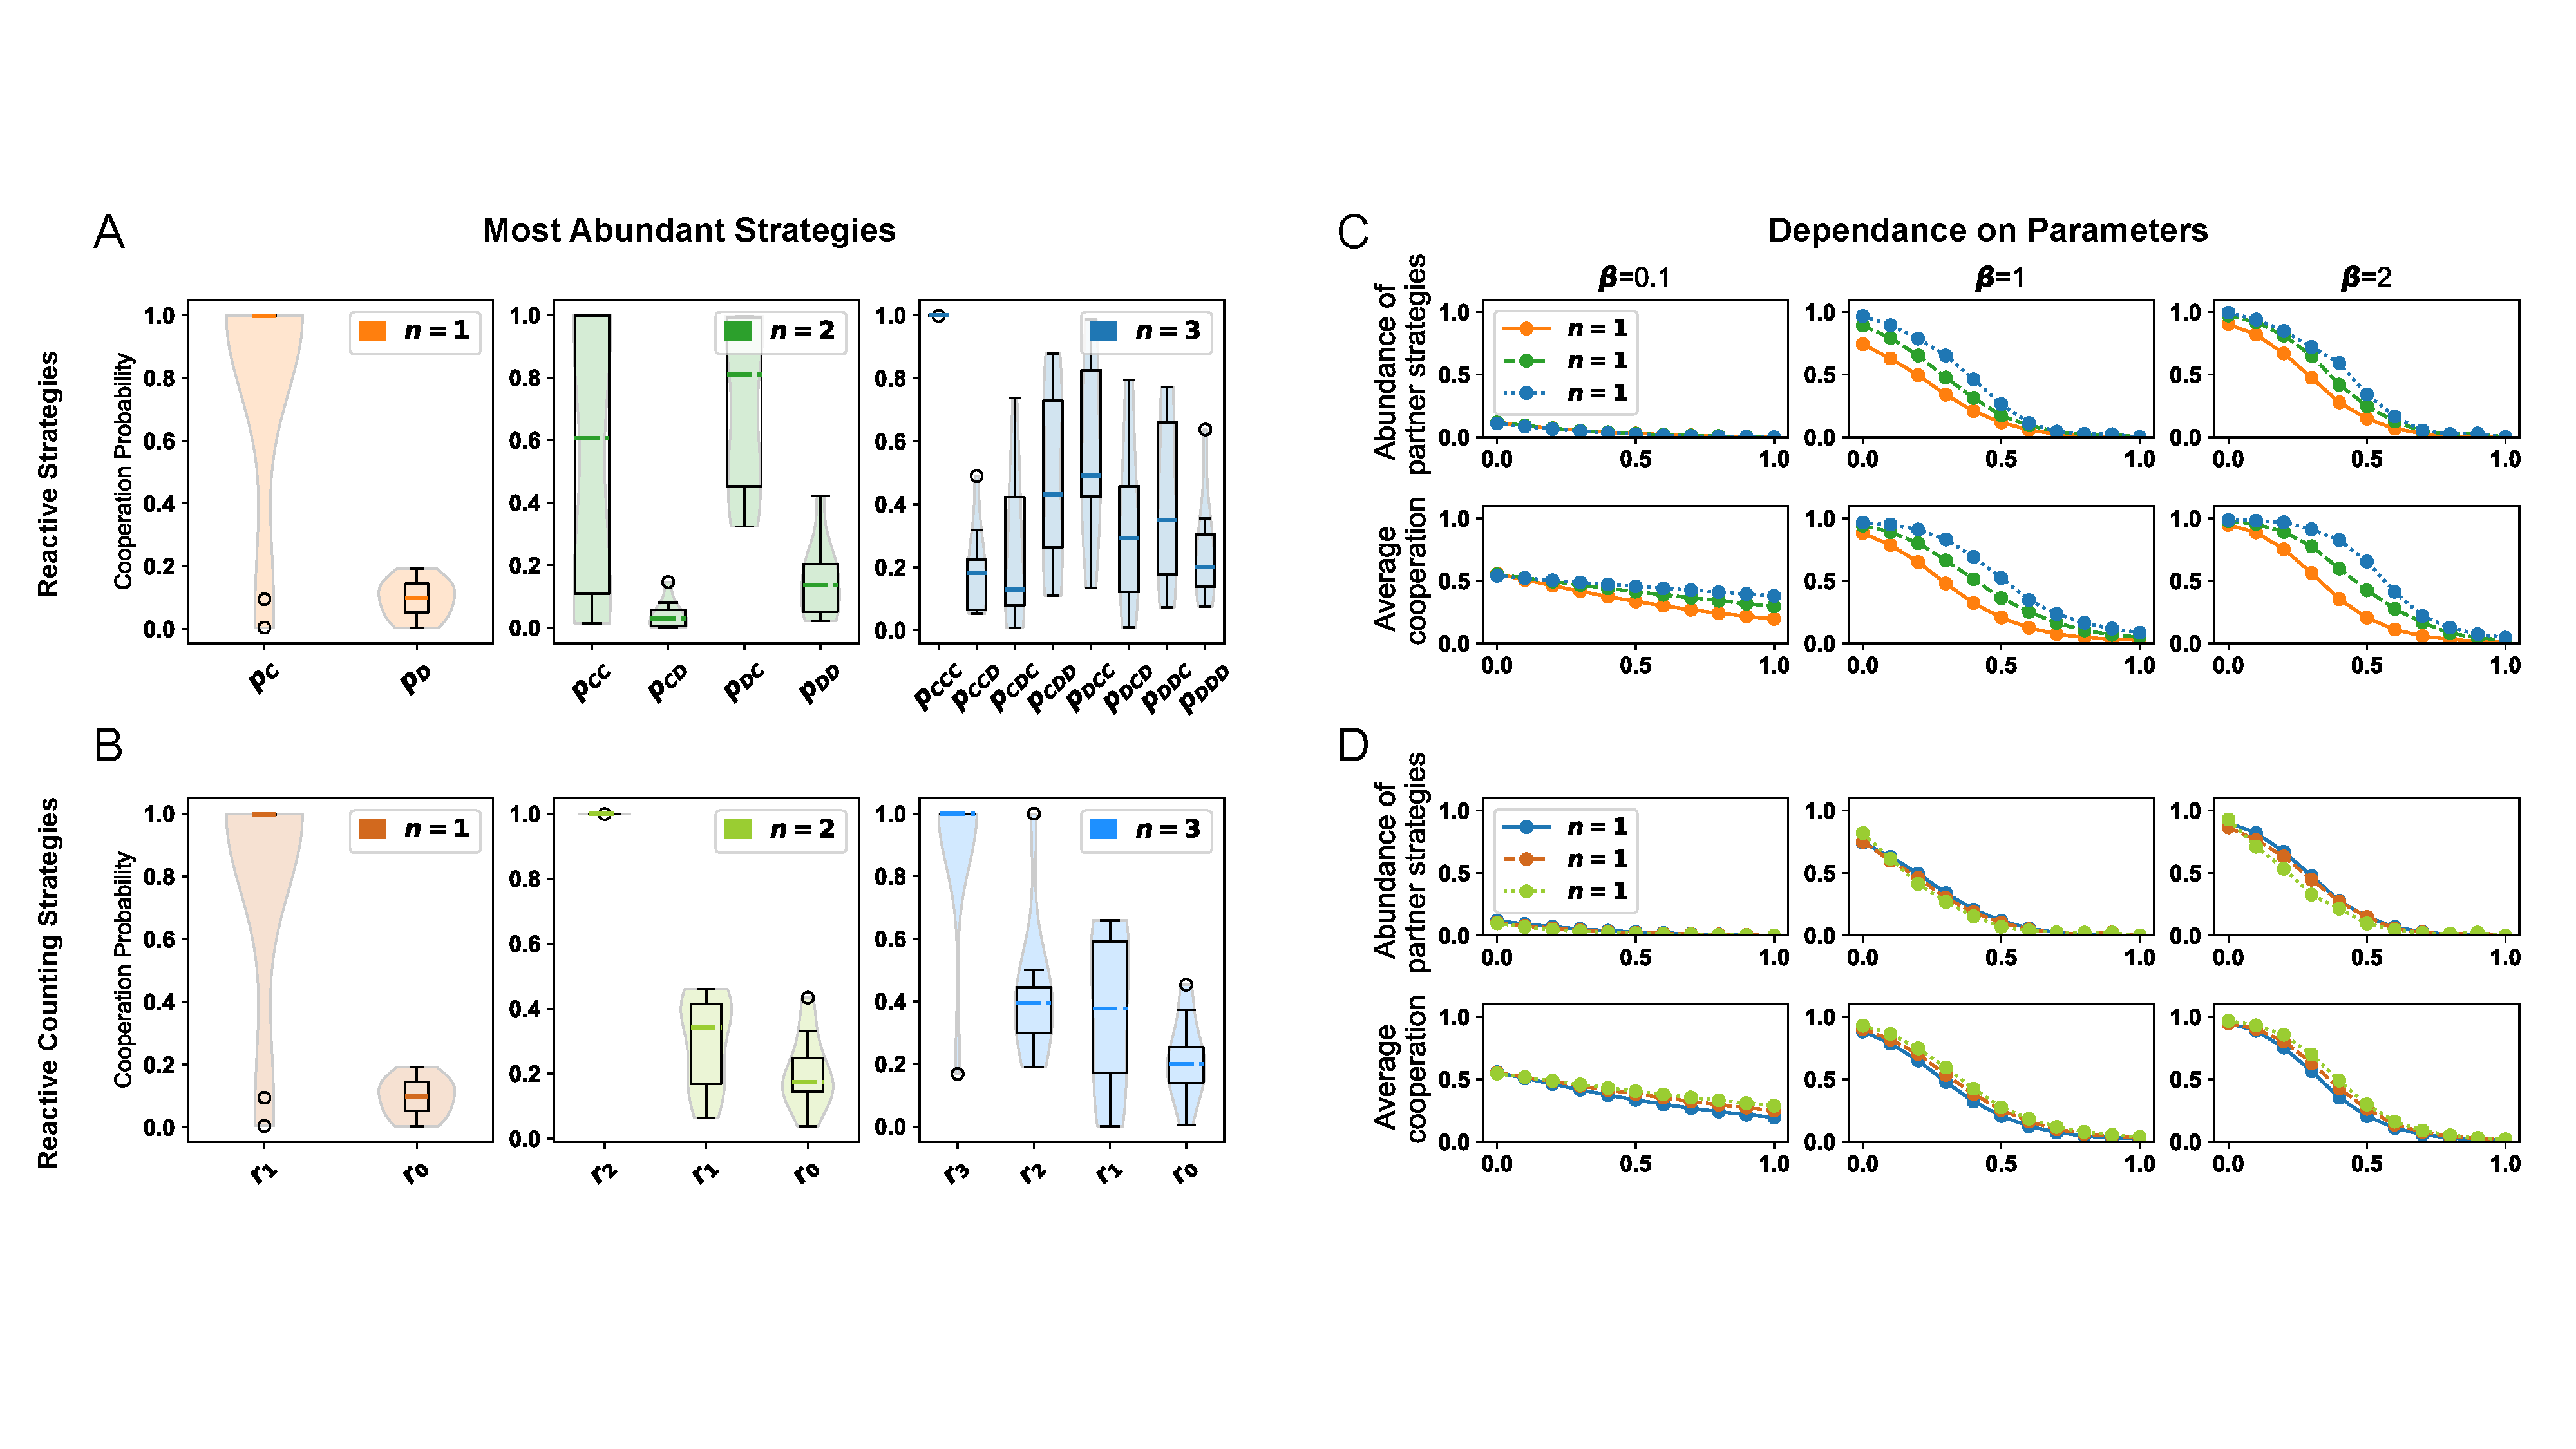
\includegraphics[width=\textwidth]{figures/evolutionary_results.pdf}
  \caption{\textbf{Evolutionary Dynamics in the Space of Reactive Strategies.}
  In the preceding sections, we characterized partner strategies for reactive$-2$
  and reactive$-3$. Additionally, we discussed the case of reactive counting
  strategies. Now, our focus is on assessing whether partner strategies can evolve
  in an evolutionary context. We ran simulations based on the methodology of Imhof
  and Nowak~\cite{imhof:royal:2010}. In a single run of the evolutionary process,
  we recorded the cooperation probabilities of the resident at each elementary
  time step.
  \textbf{a-b. Most Abundant Reactive Strategies.} We performed 10 independent
  simulations for each set of strategies and documented the most abundant strategy
  for each run. The most abundant strategy is the resident that remained fixed for
  the most time steps. For these simulations, we used \(b=1 \text{ and } c=.5\).
  For $n$ equal to 1 and 2, \(T= 10 ^ 7\) and for $n=3$ then \(T= 2 \times10 ^
  7\).
  \textbf{c-d. Abundance of Partner Strategies.}
  We ran the evolutionary process once more, this time varying the cost ($c$) and
  the strength of selection ($\beta$). The cooperation benefit ($b$) remained
  fixed at a value of 1. In these simulations, our interest lies in observing how
  frequently partner strategies become the resident strategy and in assessing the
  effects of longer memory.}\label{fig:evolutionary_results}
\end{figure}


\section{Discussion}

~\\
\bibliography{bibliography.bib}

\end{document}